\section{物理モデル}
    本章ではまず結合共振回路の物理モデルの説明から始める。
\section{超伝導回路素子}
    サンプル作成に使用した超伝導回路素子の説明を包括的に行う。まずは超伝導共振器の導入を行う。
    \subsection{超伝導共振器}
        超伝導量子エレクトロニクスの分野ではしばしば共振回路が使用される。目的は様々であるが、量子ビットを外部から遮断するためのフィルターとしてや量子ビット同士を結合させるバスとしても利用される。
        \subsubsection{超伝導分布定数回路}
            最も使用頻度の高いデザインは平面型共振回路(CPW)である。CPW型共振回路の特徴は伝送ラインの断面図が任意の点で50Ωに保たれていることである。グランドラインと伝送ラインの間の溝を常に一定に保つことで共振回路長を調節するだけで共振周波数を調節することができる。この時共振回路全体のインダクタンスとキャパシタンスは単位あたりのインダクタンスLp.u.lとキャパシタンスCp.u.lを共振回路長で乗算したものである。このように回路の共振パラメータが一様に分布したモデルで記述される共振器のことを分布定数型共振回路と呼ぶ。またインピーダンス不整合が抑制されているため共振回路のQ値も特別な処理を施さずとも高い。CPW型の共振周波数がどのような物理モデルによって記述されるのかは補足に記したので参照されたい。
        \subsubsection{超伝導準集中定数回路}
            分布定数型の共振回路のデメリットはデザインに自由度がないことである。多くの超伝導素子を1つのサンプルに集積する際には回路デザインは非常に重要である。量子ビットのQ値は高く保って置きたいため、次にデザインに自由度を持たせるとすれば共振器になる。そういったケースを考えるとCPWのような共振回路では回路作成に困難を要する。
            また、共振回路同士の結合を考える場合、その結合方式は電気的結合(キャパシティブ結合)か磁気的結合(インダクティブ結合)になる。高強度の結合を考える際、結合にはどちらか一方のみを考える方が望ましい。両方の結合項を同時に記述すれば結合強度に対してそれぞれ逆符号をとっていることがわかる。今回作成したサンプルではどれもインダクティブな結合方式を利用することを考えた。
            この場合結合には電磁誘導の法則が適用されるため、結合強度を決めるパラメータは共振器間の実質的な相互インダクタンスと共振器に流れる電流に依存する。つまり共振器に流れる電流は大きい方がよい。共振回路を流れる電流は共振回路のインダクタンスを用いて以下のように記述される。つまり同一の周波数を持つ共振器において、キャパシタンス部分は小さく、インダクタンス部分が大きいことが共振器としては望ましいことがわかる。こういった調整をCPW型の共振器で行うことは難しい。局所的なパラメータを調整する際には今回採用した集中定数素子型の共振器wお使用することが理想的であるといえる。
            分布定数回路に対して共振素子のインダクタンスとキャパシタンスが部分的に集中した回路のことを集中定数素子型の共振器と呼ぶ。この場合、CPW型の共振素子とはその特性が異なる。CPW型の共振器はキャパシタンスを開放端、グランドを固定端とした空洞間に閉じ込められた音響モードと物理的には全く同じ振る舞いをする。基本モードの整数倍の共振周波数で共鳴し、両端開放型の共振器を$\lambda/2$型の共振器、開放ー固定型の共振器を$\lambda/4$型共振器と呼び、通常はそれぞれの基本モードのみを使う。
    \subsection{ジョセフソン接合}
            ジョセフソン接合は超伝導量子エレクトロニクスという研究分野の根幹をなす素子である。超伝導量子回路を構成するあらゆる素子にジョセフソン接合は使われている。使用用途は様々であるが例えば量子ビットを作成することを考える際には共振回路に非調和性をもたらす素子として導入される。前小節で述べたように共振回路の遷移周波数はすべて同一である。同一の周波数を持っていることは例えば量子ビットを作ろうと考えた時には、適していないことがわかる。量子ビットの状態をその遷移周波数で励起しても高準位の遷移周波数も同一であるためいつまでたっても励起し続けてしまうためである。
            本研究では結合素子であるrf-SQUIDを構成する素子としてジョセフソン接合を導入する。

            多方面である使用されるジョセフソン接合であるがその基本的な物理現象についてこの小節にて説明する。
            2つの超伝導体を薄い常伝導金属、半導体などを介してサンドウィッチするような接合のことを、josephson接合と呼ぶ\\
            この接合により生じる物理的現象を利用して我々は量子ビットやSQUID、その他微細デバイスを作成している。\\
            ここではjosephson接合による物理的効果を理論から解説していくこととする。

    
            この接合により生じsる物理的現象を、発見者の名に因んでjosephson効果と呼ぶ。
            この現象は大別するとACjosephson効果、DCjosephson効果の2つに分けることができる。
            この2つの効果についてGL理論から解説を始めることとする。
            \subsubsection{dc josephson効果}
                josephsonが1962年に行った理論的予言によれば、2つの超伝導体の間にゼロ電圧下で以下のような超伝導電流が流れるとしている。
                \begin{equation*}
                    I_s = I_c \sin(\Delta \psi)
                \end{equation*}
                ここで$\Delta \psi$とはGL波動関数のs位相差である。:また、臨界電流$I_c$は接合に流すことのできる、最大の超伝導電流である。
                彼はさらに接合に電位差vが生じているときに位相差が次のように振動すると予言した。
                \begin{equation*}
                    \frac{d(\Delta \psi)}{dt} = \frac{2eV}{\hbar}
                \end{equation*}
                これにより、電流は振幅を臨界電流$I_c$、周波数を$\nu = \frac{2eV}{h}$の交流となる。
                つまり、この電流変化はエネルギー$h\nu$でクーパー対が接合を通過するエネルギーと一致していることがわかる。
                以上2つの関係式によりこの接合により蓄えられるエネルギーは
                \begin{eqnarray}
                    \int_0^{t} (I_s V)dt&=&\int_{0}^{\delta} I_s(\hbar/2e)d\delta\\
                    &=&E_j(1-\cos(\delta))\\
                \end{eqnarray}
                と表現することができる。ここで$E_j=\hbar I_c/2e$である。
    \subsection{rf-SQUID}
                rf-SQUIDは
    \subsection{dc-SQUID}
        dc-SQUIDは超伝導ループ両枝にジョセフソン接合を一つずつ導入したものである。磁束量子干渉計とも呼ばれ広範囲の分野で応用されている素子である。代表的な例を上げれば重力波の観測やなどに使われている。外部磁場に非常に敏感であり
        dc-SQUIDを導入する意図はrf-SQUIDのジョセフソン接合を可変にするためである。これによりrf-SQUIDのジョセフソンインダクタンスは外部磁場に対し変化する。
        \begin{figure}[H]
            \centering
            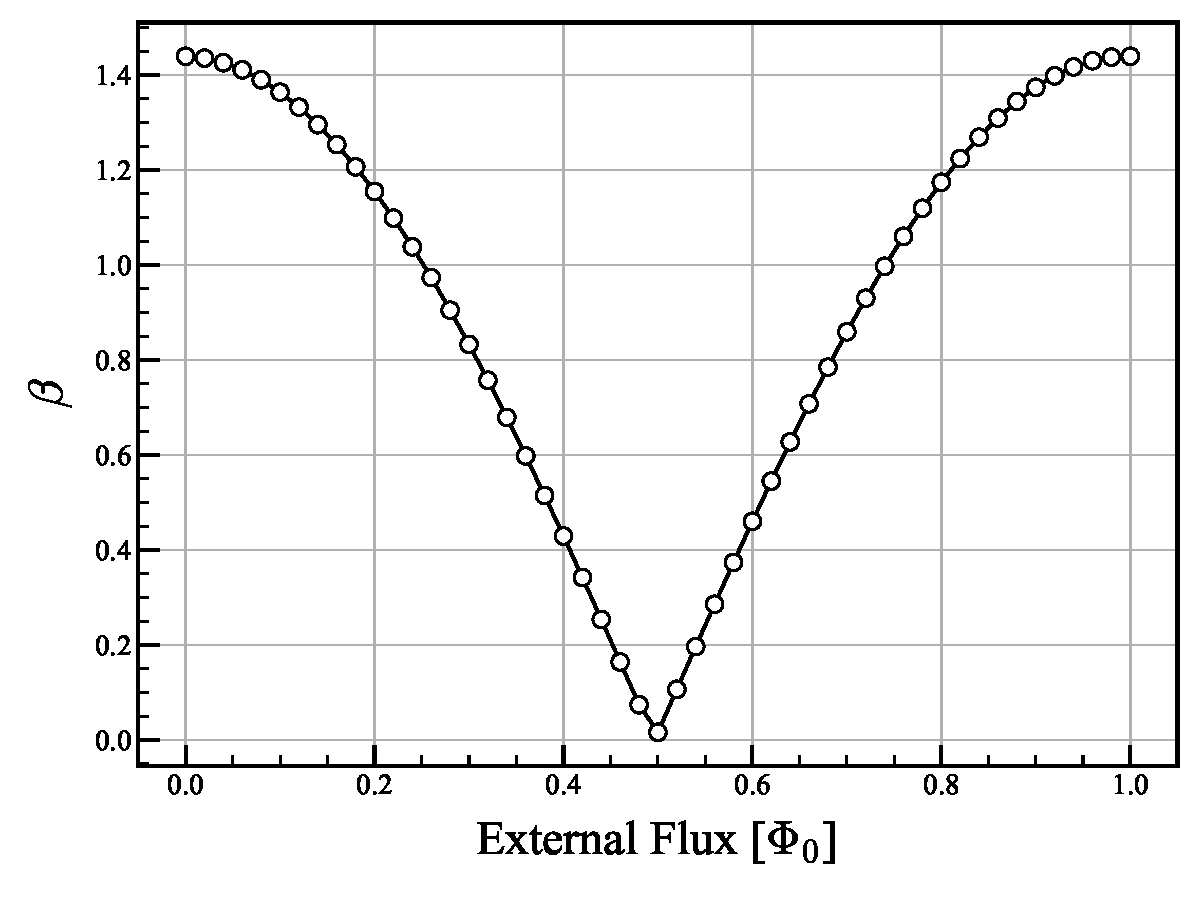
\includegraphics[width=9cm]{dc-squid.pdf}
            \caption{エネルギースペクトル}
        \end{figure}
        ではこのdc-SQUIDによってどのようジョセフソンインダクタンスが変化するのかを示す。
    \subsection{カイネティックインダクタンス}
        カイネティックインダクタンスは超伝導インダクタンスとも呼ばれる。超伝導細線を扱うとこのインダクタンスの影響が大きくなる。超伝導体中の準粒子移動により誘導されるインダクタンスである。このカイネティックインダクタンスは物質固有の値であり、非常に局所的な領域で大きなインダクタンスを得られるため、この特性を利用した量子ビットなども存在する。今回限られた設計内でおおきなインダクタンスを得るためにこのカイネティックインダクタンスを導入した。次節導入するミアンダインダクタンスは1μで加工されており、カイネティックインダクタンスの影響が大きく現れるとよそうされる。
    \subsection{ミアンダインダクタンス}
        ミアンダとは蛇行したという意味である。図の通り単純な直線ラインではなく折り返し構造を繰り返すことで、実質的な長さ、ライン間の相互インダクタンスにより総合的な自己インダクタンスが大きくなる。このミアンダインダクタンスを導入する上で論文の解析を利用した。計算方法を補足に記したので参照されたい。計算結果のみを示すと下図の構造に与えられた数値を入力することで得たいインダクタンスを求めることが可能である。次章でも言及するがこのミアンダインダクタンスの数値を考える上でもう一つ電磁界シミュレーションによる方法もとったのでここで紹介する。
        電磁界シミュレーションにはnational instruments社のマイクロウェーブオフィスを利用している。CADファイルで設定されたオブジェクトに材質特性を付与し電磁波の入出ポートを設定することで反射特性等を計算することが可能である。
        ここでシミュレーションする構造物は下図のようなミアンダインダクタンスのない単体の共振器とミアンダインダクタンスを導入した単体の共振器である。この2つのこの構造物全体のアドミッタンスを低周波数領域で計算することで構造物全体の伝導伝導性を計算することができる。アドミッタンス値からおおよその構造物のインダクタンスを計算することができるが2つの構造物の差分はおおよそミアンダインダクタンスの可否に依存する。そこでミアンダの数に対してインダクタンスがどれだけ増加するかプロットしたものが図である。この図からはミアンダの数に依存して線形にインダクタンスが増加していることがわかる。ここで上述した解析計算とどれだけの差があるかも同時にい示す。

        プロットの結果では0-100の範囲内で両者の乖離はおよそOOであった。さほど乖離はないといえるが参考値程度にとどめておく。今回のサンプル作成ではN=38をミアンダインダクタンスとして採用した。
        
        